\documentclass[12pt,a4paper]{article}
\usepackage{cmap} % Makes the PDF copiable. See http://tex.stackexchange.com/a/64198/25761
\usepackage[T1]{fontenc}
\usepackage[brazil]{babel}
\usepackage[utf8]{inputenc}
\usepackage{amsmath}
\usepackage{amsfonts}
\usepackage{amssymb}
\usepackage{amsthm}
\usepackage{textcomp} % \degree
\usepackage{gensymb} % \degree
\usepackage[usenames,svgnames,dvipsnames]{xcolor}
\usepackage{hyperref}
\usepackage{multicol}
\usepackage{graphicx}
\usepackage[margin=2cm]{geometry}
\usepackage{systeme}

\hypersetup{
    colorlinks = true,
    allcolors = {blue}
}

% TODO: Consider using exsheets
% http://linorg.usp.br/CTAN/macros/latex/contrib/exsheets/exsheets_en.pdf
%
% http://ctan.org/tex-archive/macros/latex/contrib/exercise/
% Options: answerdelayed,lastexercise,noanswer
\usepackage[answerdelayed,lastexercise]{exercise}

\addto\captionsbrazil{%
\def\listexercisename{Lista de exerc\'icios}%
\def\ExerciseName{Exerc\'icio}%
\def\AnswerName{Solu\c{c}\~ao do exerc\'icio}%
\def\ExerciseListName{Ex.}%
\def\AnswerListName{Solu\c{c}\~ao}%
\def\ExePartName{Parte}%
\def\ArticleOf{de\ }%
}

\renewcommand{\ExerciseHeaderTitle}{(\ExerciseTitle)\ }
\renewcommand{\ExerciseListHeader}{%\ExerciseHeaderDifficulty%
\textbf{%\ExerciseListName\
\ExerciseHeaderNB.\ %
%\ --- \
\ExerciseHeaderTitle}%
%\ExerciseHeaderOrigin
\ignorespaces}
\renewcommand{\AnswerListHeader}{\textbf{\ExerciseHeaderNB.\ (\AnswerListName)\ }}

\newcommand*\R{\mathbb{R}}

% Loop Space / CC BY-SA-3.0 / https://tex.stackexchange.com/a/2238/25761
\newenvironment{amatrix}[1]{%
  \left[\begin{array}{@{}*{#1}{c}|c@{}}
}{%
  \end{array}\right]
}

% Loop Space / CC BY-SA-3.0 / https://tex.stackexchange.com/a/3164/25761
%--------grstep
% For denoting a Gauss' reduction step.
% Use as: \grstep{\rho_1+\rho_3} or \grstep[2\rho_5 \\ 3\rho_6]{\rho_1+\rho_3}
\newcommand{\grstep}[2][\relax]{%
   \ensuremath{\mathrel{
       {\mathop{\longrightarrow}\limits^{#2\mathstrut}_{
                                     \begin{subarray}{l} #1 \end{subarray}}}}}}

\renewcommand{\theenumi}{\alph{enumi}}
\renewcommand\labelenumi{(\theenumi) }

\newcommand*\tipo{Prova I}
\newcommand*\turma{PRO112-02U}
\newcommand*\disciplina{ALI0001}
\newcommand*\eu{Helder G. G. de Lima}
\newcommand*\data{19/03/2018}

\author{\eu}
\title{\tipo - \disciplina}
\date{\data}

\begin{document}
\thispagestyle{empty}
\newgeometry{margin=2cm,bottom=0.5cm}
\begin{center}

\includegraphics[width=9.0cm]{marca} \\
\textbf{\tipo\ (\disciplina / \turma)} \\
Prof. \eu \footnote{
Este é um material de acesso livre distribuído sob os termos da licença \href{https://creativecommons.org/licenses/by-sa/4.0/deed.pt_BR}{Creative Commons Atribuição-CompartilhaIgual 4.0 Internacional}}
\end{center}

\noindent Nome do(a) aluno(a): \underline{\hspace{9,7cm}} Data: \underline{\data}

%\section*{Instruções}
\begin{center}\fbox{
\begin{minipage}{14cm}

{\footnotesize
\begin{itemize}
\renewcommand{\theenumi}{\Roman{enumi}}
\item Identifique-se em todas as folhas.
\item Mantenha o celular e os demais equipamentos eletrônicos desligados durante a prova.
\item Resolva (integralmente) apenas os itens de que precisar para somar 10,0 pontos.
\end{itemize}
}

\end{minipage}
}
\end{center}

\section*{Questões}
\begin{ExerciseList}
\Exercise[title={2,5}]
\begin{minipage}[t]{0.59\textwidth}
O volume de carros que circulam por hora nos entornos de uma praça no centro de uma cidade é mostrado ao lado. É possível que o tráfego nos trechos $x_1$ e $x_2$ sejam idênticos? Em caso afirmativo, obtenha os valores de $x_1$, $x_2$ e $x_3$. Justifique suas afirmações.
\end{minipage}
\hfill
\begin{minipage}[t]{0.3\textwidth}
\raggedleft\vspace{-0.25cm}
\vfill
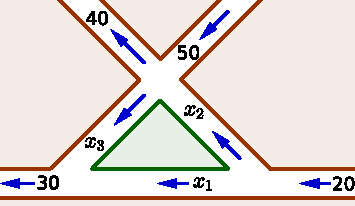
\includegraphics[width=4.6cm]{img/prova-1-pro-quadras}
\end{minipage}
\Answer Considerando que $x_1$ deve ser igual a $x_2$ e que o número de carros que entram em cada cruzamento deve ser igual ao de carros que saem, pode-se concluir que $x_1$, $x_2$ e $x_3$ devem satisfazer às seguintes equações:

$\begin{cases}
x_1 + x_2 & = 20\\
x_2 +  50 & = x_3 + 40\\
x_1 + x_3 & = 30\\
x_1 & = x_2,
\end{cases}$
ou, equivalentemente, $(x_1,x_2,x_3)$ satisfazer
\systeme[x_1x_2x_3x_4]{
 x_1 + x_2 =  20,
 x_2 - x_3 = -10,
 x_1 + x_3 =  30,
 x_1 - x_2 =   0.
}

Procedendo com o escalonamento da matriz ampliada do sistema, obtém-se:
{\footnotesize
\begin{align*}
\begin{bmatrix}
 1 &  1 &  0 &  20 \\
 0 &  1 & -1 & -10 \\
 1 &  0 &  1 &  30 \\
 1 & -1 &  0 &   0
\end{bmatrix}
\rightarrow
& \begin{bmatrix}
 1 &  1 &  0 &  20 \\
 0 &  1 & -1 & -10 \\
 0 & -1 &  1 &  10 \\
 0 & -2 &  0 & -20
\end{bmatrix}
\rightarrow
\begin{bmatrix}
 1 &  1 &  0 &  20 \\
 0 &  1 & -1 & -10 \\
 0 &  0 &  0 &   0 \\
 0 &  0 & -2 & -40
\end{bmatrix}
\rightarrow
\begin{bmatrix}
 1 &  1 &  0 &  20 \\
 0 &  1 & -1 & -10 \\
 0 &  0 & -2 & -40 \\
 0 &  0 &  0 &   0
\end{bmatrix} \\
\rightarrow
&\begin{bmatrix}
 1 &  1 &  0 &  20 \\
 0 &  1 & -1 & -10 \\
 0 &  0 &  1 &  20 \\
 0 &  0 &  0 &   0
\end{bmatrix}
\rightarrow
\begin{bmatrix}
 1 &  1 &  0 &  20 \\
 0 &  1 &  0 &  10 \\
 0 &  0 &  1 &  20 \\
 0 &  0 &  0 &   0
\end{bmatrix}
\rightarrow
\begin{bmatrix}
 1 &  0 &  0 &  10 \\
 0 &  1 &  0 &  10 \\
 0 &  0 &  1 &  20 \\
 0 &  0 &  0 &   0
\end{bmatrix}
\end{align*}
}
Portanto, o sistema é possível e determinado (pois a matriz de coeficientes e a matriz ampliada do sistema possuem posto 3, que é igual ao número de incógnitas), e $x_1 = x_2 = 10$ e $x_3 = 20$.

\Exercise[title={2,5}] Sejam $A = \begin{bmatrix}
-2 & 0 & 2\\
 1 & 0 & -1
\end{bmatrix}$ e $B = \begin{bmatrix}
-2 &  0 &  5\\
-3 & -5 &  0\\
 4 &  0 & -10
\end{bmatrix}$. Construa, realizando somente operações de adição, subtração, multiplicação por escalar, multiplicação, transposição e/ou inversão a partir das matrizes dadas, um exemplo de cada um dos seguintes tipos de matrizes:
\begin{multicols}{3}
\begin{enumerate}
\item Simétrica ($\neq 0$)
\item Triangular inferior ($\neq 0$)
\item Inversível
\end{enumerate}
\end{multicols}
\Answer
\begin{enumerate}
\item A soma ou o produto de uma matriz com sua transposta (à esquerda ou à direita) sempre é uma matriz simétrica (por quê?). Disto resultam os seguintes exemplos:
\[
B + B^T
=\begin{bmatrix}
-4 & -3 & 9\\-3 & -10 & 0\\9 & 0 & -20
\end{bmatrix},\quad
A \cdot A^T
=\begin{bmatrix}
8 & -4\\-4 & 2
\end{bmatrix},\quad
A^T \cdot A
=\begin{bmatrix}
5 & 0 & -5\\0 & 0 & 0\\-5 & 0 & 5
\end{bmatrix},
\]
\[
B \cdot B^T
=\begin{bmatrix}
29 & 6 & -58\\6 & 34 & -12\\-58 & -12 & 116
\end{bmatrix},\quad\text{ou}\quad
B^T \cdot B
=\begin{bmatrix}
29 & 15 & -50\\15 & 25 & 0\\-50 & 0 & 125
\end{bmatrix}.
\]
\item Usando a matriz $A^T\cdot A$ obtida no item anterior, que é quase triangular inferior, exceto pelo termo -5 da primeira linha, obtém-se:
\[
(A^T\cdot A) + B = 
\begin{bmatrix}
5 & 0 & -5\\0 & 0 & 0\\-5 & 0 & 5
\end{bmatrix}
+
\begin{bmatrix}
-2 &  0 &  5\\
-3 & -5 &  0\\
 4 &  0 & -10
\end{bmatrix}
=
\begin{bmatrix}
 3 &  0 &  0\\
-3 & -5 &  0\\
-1 &  0 & -5
\end{bmatrix}.
\]
\item Como a matriz $(A^T \cdot A) + B$ é triangular inferior, $\det{((A^T \cdot A) + B)} = 3 \cdot(-5)\cdot(-5) \neq 0$ e, portanto, $(A^T \cdot A) + B$ é inversível. Outro exemplo é $B + B^T$, pois $\det{B + B^T} = 190 \neq 0$.

\textbf{Obs.:} uma vez verificado que $\det{B} = 0$, poderiam ser descartados quaisquer exemplos que fossem o produto de $B$ (ou sua transposta) por alguma outra matriz (tais como $B^T\cdot B$ e $B\cdot B^T$), ou que fossem da forma $k B$ ou $k B^T$, para algum $k \in \R$, pois também teriam determinante igual a zero (afinal, $\det{BX} = \det{B}\det{X} = 0 \det{X} = 0$ e $\det{k}B = k^3 \det{B} = k^3\cdot 0 = 0$). Além disso, $A\cdot A^T$, $A^T\cdot A$, também têm determinante nulo, então também não servem.
\end{enumerate}


\Exercise[title={2,5}]
Prove (não exemplifique) se for verdadeiro, e dê um contraexemplo se for falso:
\begin{enumerate}
\item Uma matriz $m \times n$ em que todas as entradas são iguais só pode ter posto $1$ ou $0$.
\item O produto de uma matriz antissimétrica por sua transposta também é antissimétrica.
\item O produto de duas matrizes inversíveis de mesma ordem sempre é uma matriz inversível.
\end{enumerate}
\Answer
\begin{enumerate}
\item \textbf{Verdadeiro}. Seja $A$ uma matriz $m \times n$ em que todas as entradas são iguais a $k$. Se $k = 0$ então $A = 0_{m\times n}$, que tem posto zero. Caso contrário, ao subtrair a primeira linha de cada uma das linhas subsequentes obtém-se:
\[
A =
\begin{bmatrix}
k & k & \ldots & k\\
k & k & \ldots & k\\
\vdots & & \ddots & \vdots\\
k & k & \ldots & k
\end{bmatrix}
\rightarrow
\begin{bmatrix}
k & k & \ldots & k\\
0 & 0 & \ldots & 0\\
\vdots & & \ddots & \vdots\\
k & k & \ldots & k
\end{bmatrix}
\rightarrow\cdots
\rightarrow
\begin{bmatrix}
k & k & \ldots & k\\
0 & 0 & \ldots & 0\\
\vdots & & \ddots & \vdots\\
0 & 0 & \ldots & 0
\end{bmatrix}
\]
Neste caso, como a primeira linha é diferente de zero, o posto de $A$ é igual a um.
\item \textbf{Falso}. Embora $(A \cdot A^T)^T = A\cdot A^T$ seja simétrica, ela não é necessariamente antissimétrica, mesmo que $A$ seja antissimétrica. Por exemplo, tomando
$A = \begin{bmatrix}
0 & 1 \\ -1 & 0
\end{bmatrix}$
tem-se:
\[
A \cdot A^T= \begin{bmatrix}
0 & 1 \\ -1 & 0
\end{bmatrix}
\cdot
\begin{bmatrix}
0 & -1 \\ 1 & 0
\end{bmatrix}
=\begin{bmatrix}
1 & 0 \\ 0 & 1
\end{bmatrix}
\neq
\begin{bmatrix}
-1 & 0 \\ 0 & -1
\end{bmatrix}
=-A \cdot A^T
\]
\textbf{Obs.:} Isso não quer dizer que não exista alguma matriz antissimétrica $M$ tal que $M \cdot M^T$ seja antissimétrica. De fato, uma matriz nula $n \times n$ tem essa propriedade.

\item \textbf{Verdadeiro}. Se $A$ e $B$ são matrizes $n \times n$ inversíveis, então existem as matrizes $A^{-1}$ e $B^{-1}$ tais que $A A^{-1} = I =A^{-1} A$ e $B B^{-1} = I = B^{-1} B$. Então
\[
(AB) (B^{-1}A^{-1})
= A(B B^{-1})A^{-1}
= A I A^{-1}
= A A^{-1}
= I.
\]
Ou seja, $AB$ é inversível, e sua inversa é a matriz $B^{-1}A^{-1}$.
\end{enumerate}

\Exercise[title={2,5}]
Quais são as matrizes $Q$ de ordem $2 \times 2$ que satisfazem a equação $(Q + 3Q^T)^{-1} = \frac{1}{4}Q^{-1}$? Descreva esse conjunto de matrizes explicitamente, e justifique sua resposta.
\Answer Se $(Q + 3Q^T)^{-1} = \frac{1}{4}Q^{-1} = (4Q)^{-1}$ então $Q + 3Q^T = 4Q$, isto é, $3Q^T = 4Q - Q = 3Q$, ou ainda, $Q^T = Q$. Assim, as matrizes que satisfazem a condição dada são as matrizes simétricas inversíveis.

\Exercise[title={2,5}] Calcule $\det{(M \cdot M^T \cdot M^{-1})}$, sendo
$M = \begin{bmatrix}
 0 & 0 & 2 &  3\\
 1 & 0 & 0 & -1\\
-2 & 1 & 0 &  0\\
 2 & 1 & 3 &  0
\end{bmatrix}$. \textbf{Dica:} é menor do que 10.
\Answer Pelas propriedades do determinante, resulta que
\[
\det{(M \cdot M^T \cdot M^{-1})}
=\det{M} \cdot \det{(M^T)} \cdot \det{(M^{-1})}
=\det{M} \cdot \det{M} \cdot \frac{1}{\det{M}}
=\det{M}.
\]
Então,
\[
\det{(M \cdot M^T \cdot M^{-1})}
= \begin{vmatrix}
 0 & 0 & 2 &  3\\
 1 & 0 & 0 & -1\\
-2 & 1 & 0 &  0\\
 2 & 1 & 3 &  0
\end{vmatrix}
=2
 \begin{vmatrix}
 1 & 0 & -1\\
-2 & 1 &  0\\
 2 & 1 &  0
\end{vmatrix}
-3
 \begin{vmatrix}
 1 & 0 & 0\\
-2 & 1 & 0\\
 2 & 1 & 3
\end{vmatrix}
=2\cdot (2+2)-3\cdot(3)
=-1.
\]
O mesmo resultado seria obtido caso fossem realizadas operações elementares sobre as linhas da matriz $M$ para obter transformá-la em uma matriz triangular superior, cujo determinante seria o produto das entradas da diagonal.

%\Exercise[title={0,5}]\textbf{(BONUS)} Entregar atividade introdutória  sobre espaços vetoriais na próxima aula.
%\Answer \ldots
\end{ExerciseList}

\begin{center}
BOA PROVA!
\end{center}

\newpage
\restoregeometry
\section*{Respostas}
\shipoutAnswer
\end{document}
